\subsection{Background}
\begin{frame}{The system}
\begin{columns}
\column{0.7\textwidth}
Terpene Synthase \enquote{(+)-Bornyl Diphosphate Synthase}
\begin{itemize}
	\item 4511 Atoms (Not including solvent or ligand)
	\item Dynamical system that exists at room temp.
	\item Protein is not in isolation (Needs solvent)
	\item Reactions can require nanosecond simulation lengths
\end{itemize}
\vspace{1cm}
Therefore DFT or ab-initio methods are too expensive!
Molecular dynamics is therefore a much more sensible option.
\column{0.3\textwidth}
\begin{figure}
\includegraphics[width=\textwidth]{figures/System/1n23Render.png}
\end{figure}

\end{columns}
\end{frame}


\begin{frame}{The ligand}
\begin{figure}
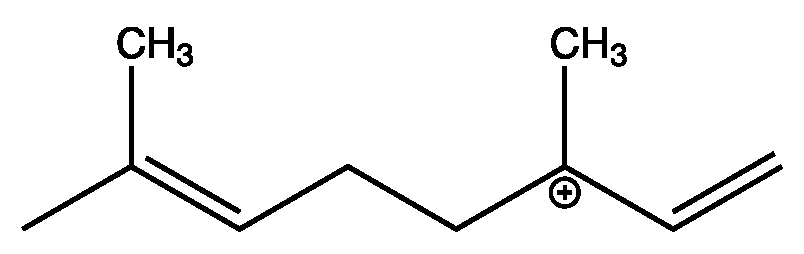
\includegraphics[height=0.3\textheight]{../Graphics/1n20Lig.eps}
\end{figure}
\begin{itemize}
\item	Initial intermediate Geranyl Diphosphate - Bornyl Diphosphate synthetic route
\item	Monoterpene carbocation
\item	Natural ligand for this protein 
\item	Unsaturated 
\end{itemize}
\end{frame}

